\chapter{Project Overview}
The key features of the application are introduced in this chapter. The system is described primarily from the perspective of the user, as the back-end processes are focused on in later chapters of this report. 

\section{Features}
The web application is a contained within a single page, that is, all POST and GET requests do not result in a redirect, but instead dynamically update to reflect new data. A user will start by entering a text query into the form, and pressing 'search' (Figure \ref{screen1}). 

\begin{figure}[!ht]
\begin{center}
	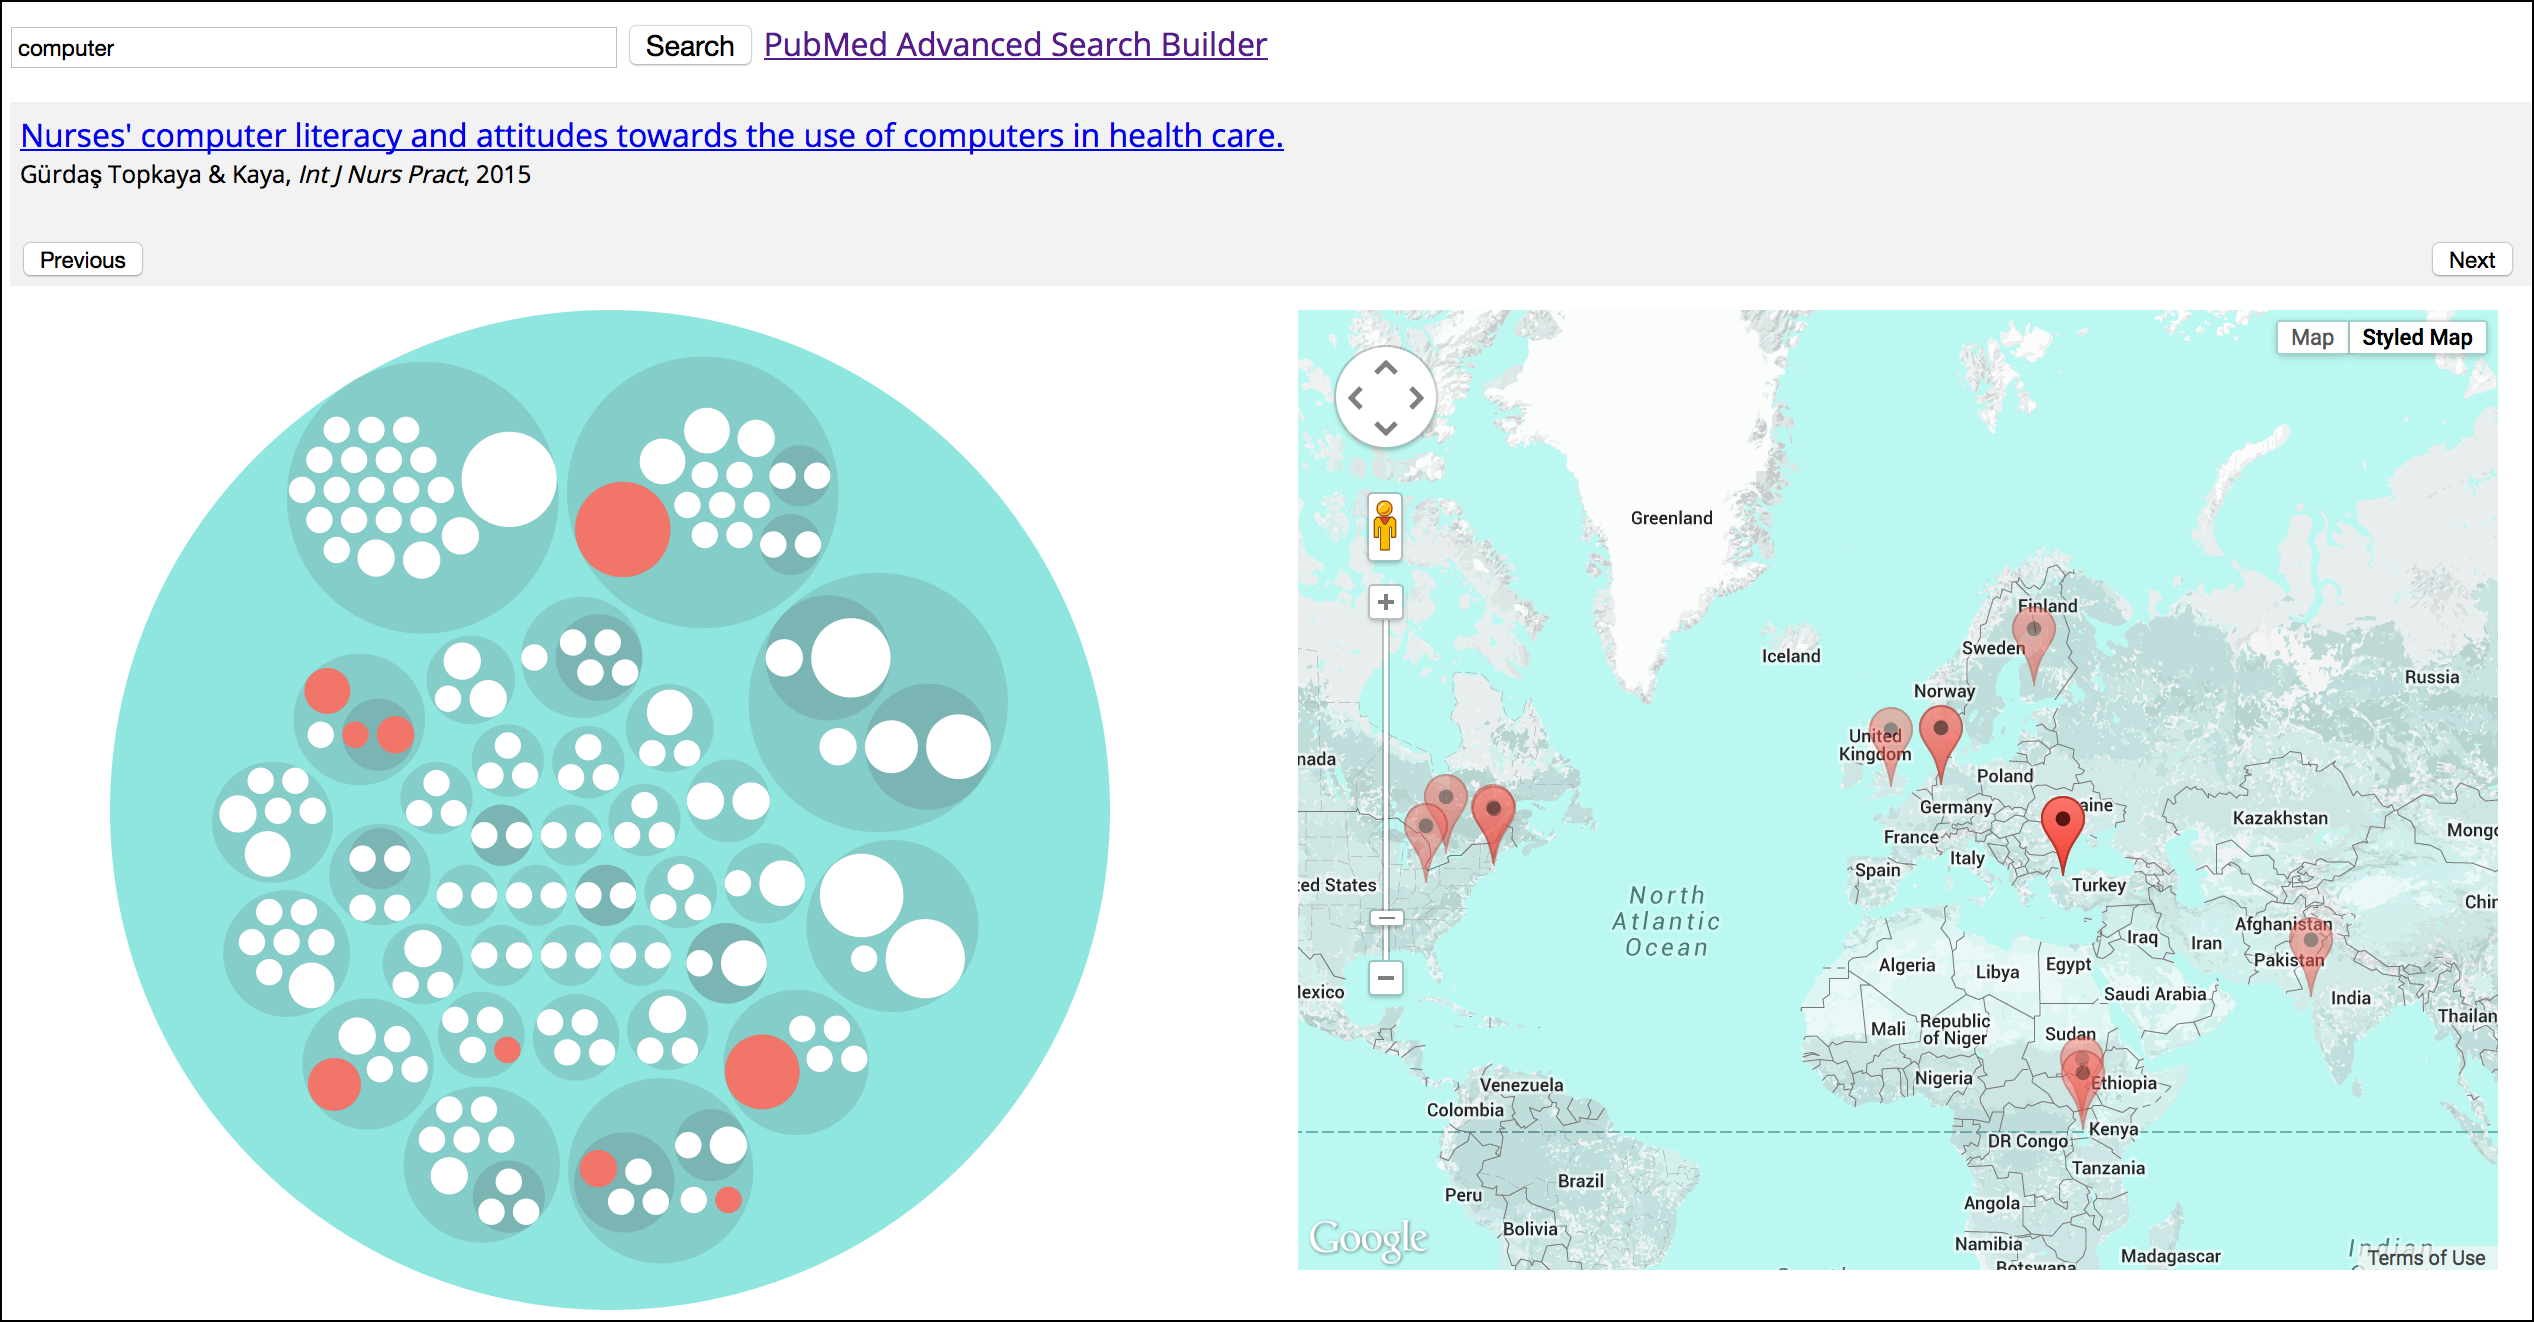
\includegraphics[width=0.8\textwidth]{../lib/images/screen1}
	\caption{Box and Whisker diagrams for 3 formats with balanced hit rates and accuracies. Key values have been added to the diagram to allow clearer comparison, as the y-axis is log10 scale.\label{fig:geoboxes}}
\end{center}
\end{figure}


EVALUATION
query 'computer' before cache: 
BEGIN 2015-09-04 21:50:57.860764
END 2015-09-04 21:55:55.429222
BEGIN 2015-09-04 21:58:27.498693
END 2015-09-04 21:58:37.515853
query 'computer' after cache: 